\subsection*{\textbf{Задание 11.1} Набор выражений.}
Наберите в документе следующее выражение:
$45*x+(50*39/99)*x/5+7!*8*x^2/8!+Sqrt[34*x^4]$
нажмите \textbf{[Shift] + [Enter]} для вывода результата.
Введите выражение $x*(y^2-z^2)+y*(z^2-x^2)+z(x^2-y^2)$
упростите это выражение, нажав \textbf{[Shift] + [Enter]}.

\begin{figure}[H]
    \renewcommand{\figurename}{Рисунок}
    \centering{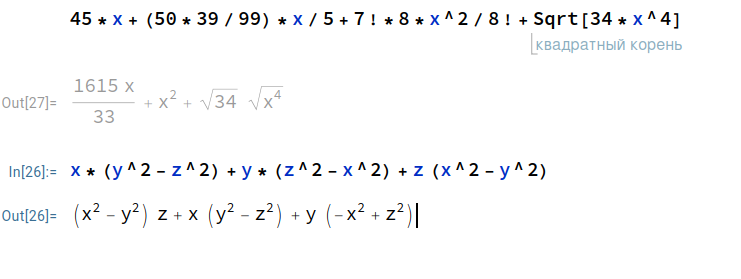
\includegraphics[scale=0.70]{body/img/1.png}}
    \label{fig:image_1}
\end{figure}